% Authoritative complete manuscript. Edit paper/main.tex directly.
% All prose, equations, tables, result macros and bibliography are inline.
% Source comments record provenance, not build dependencies.
% External assets: official LLNCS class/packages and the six figure PDFs.
\documentclass[runningheads]{llncs}
\usepackage[T1]{fontenc}
\usepackage{lmodern}
\usepackage{microtype}
\usepackage{amsmath,amssymb,booktabs,graphicx,tabularx,array}
\usepackage[hidelinks]{hyperref}
\hypersetup{pdftitle={Semantic Structure and Revision in Temporal Evidence Graphs for Generative Monitoring},pdfauthor={Anonymous}}
\graphicspath{{../artifacts/figures/}}
\newcommand{\method}{M1}
% start input ./generated/macros.tex
% Generated from saved completed runs.
\newcommand{\TotalInitial}{3,600}
\newcommand{\TotalRepairs}{1,620}
\newcommand{\TotalRequests}{5,220}
\newcommand{\PilotInteractivePFifty}{13.34}
\newcommand{\PilotInteractivePNinetyFive}{17.07}
\newcommand{\PilotBatchRate}{0.323}
\newcommand{\TotalFailed}{3}
\newcommand{\TotalTruncated}{0}
\newcommand{\TotalInitialErrors}{3}
\newcommand{\ClientTimeouts}{0}
\newcommand{\UsageUnavailable}{3}
\newcommand{\BaselineInvalidClaims}{799}
\newcommand{\OffTargetSupportedClaims}{333}
\newcommand{\MainHours}{2.89}
\newcommand{\AuditFlagged}{4}
\newcommand{\AuditParsed}{60}
\newcommand{\AuditDisagreements}{14}
\newcommand{\AuditCalibration}{4}
\newcommand{\GraphParentClaims}{18}
\newcommand{\GraphTotalClaims}{1201}
\newcommand{\SystemsCalls}{472}
\newcommand{\SystemsExplanations}{236}
\newcommand{\SystemsAdequate}{0}
\newcommand{\SystemsWithoutDifference}{236}
\newcommand{\AuditAcceptedInvalid}{10}
\newcommand{\AuditFlaggedValid}{4}
\newcommand{\GraphFlagMisses}{21}
\newcommand{\GraphRepairMisses}{40}
\newcommand{\SystemsRepairTargets}{40}
 % end input ./generated/macros.tex
 % start input ./generated/semantic/macros.tex
\newcommand{\SemParentClaims}{18}
\newcommand{\SemDisplayedClaims}{1201}
\newcommand{\SemParentlessPercent}{98.5}
\newcommand{\SemExportScopes}{480}
\newcommand{\SemVerifiedPaths}{1850}
\newcommand{\SemStorageNodes}{47,038}
\newcommand{\SemStorageEdges}{128,789}
\newcommand{\SemBackground}{333}
\newcommand{\SemInvalidGrounded}{499}
\newcommand{\SemContractInvalid}{799}
\newcommand{\SemRevisionBatches}{360}
\newcommand{\SemEligibleBatches}{210}
\newcommand{\SemNonzeroExposure}{0}
\newcommand{\SemLocalityViolations}{0}
\newcommand{\SemCoreCalls}{325}
\newcommand{\SemCoreRepairs}{85}
\newcommand{\SemCoreCases}{240}
\newcommand{\SemCoreRoots}{209}
\newcommand{\SemCoreMinutes}{17.2}
\newcommand{\SemReplayCells}{9,600}
\newcommand{\SemPredictionGroups}{860}
\newcommand{\SemPredictionAgreement}{860}
\newcommand{\SemParityGroups}{1,920}
\newcommand{\SemSameSize}{236}
\newcommand{\SemRootOne}{74}
\newcommand{\SemRootTwo}{135}
\newcommand{\SemMissingRoots}{31}
\newcommand{\SemAliasRoots}{229}
\newcommand{\SemAliasCells}{4,800}
\newcommand{\SemAliasRequired}{1294}
\newcommand{\SemAliasMissed}{208}
\newcommand{\SemUnknownPrimitive}{236}
\newcommand{\SemCoreSizeMin}{2.8}
\newcommand{\SemCoreSizeMax}{4.1}
\newcommand{\SemCoreRatioMin}{1.5}
\newcommand{\SemCoreRatioMax}{2.2}
\newcommand{\SemAssessmentTies}{432}
\newcommand{\SemAssessmentConflicts}{245}
\newcommand{\SemFixtureRequired}{1260}
\newcommand{\SemFixtureMissed}{720}
\newcommand{\SemFixtureAlternative}{120}
\newcommand{\SemGeneratedRequired}{1210}
\newcommand{\SemGeneratedMissed}{183}
\newcommand{\SemGeneratedAlternative}{96}
\newcommand{\SemSyntheticRawP}{87.3}
\newcommand{\SemSyntheticRawR}{95.0}
\newcommand{\SemSyntheticDisplayP}{100.0}
\newcommand{\SemSyntheticDisplayR}{78.2}
\newcommand{\SemWesadRawP}{83.4}
\newcommand{\SemWesadRawR}{87.0}
\newcommand{\SemWesadDisplayP}{100.0}
\newcommand{\SemWesadDisplayR}{75.8}
\newcommand{\SemPpgRawP}{84.7}
\newcommand{\SemPpgRawR}{88.8}
\newcommand{\SemPpgDisplayP}{100.0}
\newcommand{\SemPpgDisplayR}{75.5}
\newcommand{\SemCompetencyWitnesses}{1201}
\newcommand{\SemCompetencyComparisons}{18}
 % end input ./generated/semantic/macros.tex
 % start input ./generated/review_views/macros.tex
\newcommand{\ViewRealBefore}{1306.01}
\newcommand{\ViewRealAfter}{1336.01}
\newcommand{\ViewRealEligible}{20}
\newcommand{\ViewRealNodes}{7}
\newcommand{\ViewStructEligible}{87}
\newcommand{\ViewStructNodes}{12}
\newcommand{\ViewStructBefore}{2301.01}
\newcommand{\ViewStructAfter}{2331.01}
\newcommand{\ViewStructDepth}{2}
\newcommand{\ViewStructRequested}{2}
\newcommand{\ViewRouteAInterval}{2270--2300}
\newcommand{\ViewRouteBInterval}{2150--2270}
\newcommand{\ViewRouteOld}{5.3749}
\newcommand{\ViewRouteNew}{4.2143}
\newcommand{\ViewRouteThreshold}{4.7411}
 % end input ./generated/review_views/macros.tex
 % start input ./generated/classic_network/macros.tex
\newcommand{\ClassicNodes}{14}
\newcommand{\ClassicEdges}{18}
\newcommand{\ClassicCore}{11}
\newcommand{\ClassicContext}{3}
\newcommand{\ClassicScopeNodes}{26}
\newcommand{\ClassicScopeEdges}{83}
\newcommand{\ClassicDependencyNodes}{13}
\newcommand{\ClassicDependencyEdges}{10}
\newcommand{\ClassicInputVersions}{2}
\newcommand{\ClassicReach}{4}
\newcommand{\ClassicReachClaims}{2}
\newcommand{\ClassicChanged}{1}
\newcommand{\ClassicRequired}{1}
\newcommand{\ClassicDirect}{1}
\newcommand{\ClassicExposure}{0.0}
\newcommand{\ClassicBefore}{2301.01}
\newcommand{\ClassicAfter}{2331.01}
\newcommand{\ClassicArrival}{2331.0}
\newcommand{\ClassicOldValue}{5.374856}
\newcommand{\ClassicNewValue}{4.214302}
\newcommand{\ClassicThreshold}{4.74108975}
 % end input ./generated/classic_network/macros.tex
 \renewcommand{\topfraction}{.95}
\renewcommand{\textfraction}{.05}
\renewcommand{\floatpagefraction}{.65}
\begin{document}
\title{Semantic Structure and Revision in Temporal Evidence Graphs for Generative Monitoring}
\titlerunning{Semantic Structure and Revision}
\author{Anonymous Authors}
\authorrunning{Anonymous Authors}
\institute{Anonymous Institution}
\maketitle
\begin{abstract}
% start input ./generated/semantic/abstract.tex
Generated explanations can remain plausible after their evidence changes.
We study a typed temporal property graph that records observations, proposed
propositions, declared prerequisites and support at each knowledge time.
A query-specific semantic core retains numerical witnesses and version history.
A shared network view lets readers inspect original citations, corrected versions
and alternative support routes in the paper and dashboard. Two conditional results
bound which claims may change and characterize when direct maintenance misses
required updates. We measure these misses through transitive exposure, the fraction
of necessary changes excluded by direct scheduling. In synthetic, WESAD and
PPG-DaLiA experiments, only \SemParentClaims{} of \SemDisplayedClaims{} displayed
claims declare parents. Every eligible waveform revision has zero exposure.
Independent scoring separates source grounding from task completeness.
Checked displays are fully grounded, but subject-averaged required recall is
\SemPpgDisplayR--\SemSyntheticDisplayR\%. Across \SemCoreCases{} controlled
structural cases, exact and GPU-generated programs expose necessary intermediate
dependencies and surviving alternatives. Exposure predicts direct-maintenance
misses in all \SemPredictionGroups{} eligible replays. Full maintenance agrees
across Neo4j and an indexed relational control. Generated answers reach
evidence-to-answer depth one or two despite requests up to four.
These results explain when explicit semantic structure enables selective revision.
Storage size, path length and contract acceptance alone do not establish
explanation fidelity or maintenance benefit.
 % end input ./generated/semantic/abstract.tex
 \keywords{Temporal knowledge graphs \and Evidence provenance \and Generative explanations \and Incremental maintenance \and Physiological streams}
\end{abstract}
% start input ./sections/introduction.tex
\section{Introduction}

A generated explanation can become misleading when a sensor window is corrected,
a feature fails a quality check, or a delayed observation replaces a statement
of absence. Deleting the answer discards useful information. Keeping it may
preserve a wrong number. A temporal evidence graph records what the answer
asserted, which observations and prerequisites it cited, and what was known when.

A comparison may cite both a parent claim and the two operands directly.
Revising either operand then reaches the comparison in one step.
If an answer relies only on an intermediate claim, however, a direct checker
may update that claim and leave the answer unchanged. A reached claim may also
remain supported because another valid route survives. Understanding these
cases requires the meaning of the edges and support rules, not visual complexity.

We study a typed temporal property graph whose schema is specified by the
researcher and whose instances record provenance and generated propositions.
First, we define how the graph is constructed
and how a query selects a semantic core linked to the stored objects.
A shared network view lets a reviewer inspect original citations, version changes
and groups of supporting inputs in the paper and an evidence-review dashboard.
Second, we connect an explicit support model to a locality result and a measurable
condition under which direct and transitive maintenance agree. Third, we test
that connection using actual Neo4j exports, independent proposition scores and
a controlled structural extension of three completed benchmarks. The graph
records commitments made by the answer, not the model's internal neural reasoning.

The waveform study provides a useful contrast. Only \SemParentClaims{}
of \SemDisplayedClaims{} claims displayed by transitive graph maintenance (M1)
declare parents, and direct checking
matches transitive maintenance. Every eligible waveform revision batch has zero
transitive exposure. A separate scoring protocol distinguishes accurate background
statements from violations of the original target-only output contract. It reveals
how checking trades coverage of required facts for grounded content. We then vary
dependency depth and alternative support routes in exact numerical programs and
common GPU-generated candidates over the same recordings. Together, these results
show when propagation matters and when direct maintenance suffices.

\subsection{Relation to Prior Work}

Truth-maintenance systems revise justified beliefs when their premises
change~\cite{doyle1979}. Incremental view maintenance updates database results
when their inputs change~\cite{gupta1993}. Provenance semirings distinguish
jointly required inputs from alternative derivations~\cite{green2007}.
We connect these established ideas to the dependencies a bounded generator
actually expresses and to independently measured maintenance outcomes.

PROV-DM distinguishes entities, activities, derivation, revision and
attribution~\cite{prov2013}. It informs our separation of recording provenance,
generated assertions and review events. We implement a property graph with
Python admission checks and database identity constraints. GraphRAG builds entity
graphs and community summaries for corpus-level question answering~\cite{edge2025}.
Graphiti, described in the Zep architecture, maintains temporal information for
agent memory~\cite{rasmussen2025}. Our unit of evaluation is a revisable numerical
proposition and its admissible supporting inputs. We measure whether evidence
grounds that proposition. This differs from asking whether a model's account of
its own computation faithfully describes its decision process~\cite{turpin2023}.
 % end input ./sections/introduction.tex
 % start input ./sections/method.tex
\section{A Typed Temporal Semantic Representation}
\label{sec:representation}

\subsection{Schema-Guided Ontology Instantiation}

The ontology is fixed in code and specifies the allowed objects and relationships.
The generator proposes instances within this vocabulary. Formally, let
\begin{equation}
\begin{split}
 \Omega&=(\mathcal T,\mathcal R,\operatorname{dom},\operatorname{ran},\mathcal C),\\
 G_t&=(V_t,E_t,\vartheta_V,\vartheta_E,a_t).
\end{split}
\label{eq:ontology}
\end{equation}
Here $\mathcal T$ and $\mathcal R$ are the node and relation vocabularies.
$\vartheta_V:V_t\to\mathcal T$ and $\vartheta_E:E_t\to\mathcal R$
assign their types. An edge of type $r$ connects allowed types in
$\operatorname{dom}(r)$ and $\operatorname{ran}(r)$. Attributes $a_t$ record
immutable and logical IDs, dataset, subject, session, event interval, ingestion
time, version, value, unit and evidence state. Constraints $\mathcal C$ require
immutable identifiers, finite acyclic declared dependencies and the admission
checks below. Ingestion time $\tau_v$ is distinct from the type maps $\vartheta$.
At knowledge time $t$, only records with $\tau_v\leq t$ are visible.
Assessments become visible at their recorded knowledge time.
Queries select the greatest version visible at their knowledge time,
using ingestion time and ID to break ties. Historical queries retain that time. Tied assessments retain their trigger IDs. Conflicting states
remain ambiguous because the timestamp does not establish the order of triggers.

Table~\ref{tab:objects} lists the stored objects. Observation windows carry hashes,
sample indices and channel metadata, while raw arrays remain outside the database.
Features carry units, extractor metadata and source IDs. The
\texttt{with\_entities} function adds subject and channel identities.
The model proposes proposition fields, evidence references, parent links and
sentences. Claims that pass the bounded checks are inserted immutably.
The Neo4j adapter adds \texttt{SupportAssessment} nodes and
\texttt{ASSESSED\_AS} edges to the storage totals.
Inserting an edge can create a placeholder for an unresolved source Record.
None occurs in the original exports. Table~\ref{tab:relations} gives relation
meanings and creation rules. Neo4j enforces unique scope/ID pairs.
Python checks record kinds, immutable payloads, acyclicity and numerical
admission. The database itself does not enforce these semantic checks.

\begin{table}[!htbp]
\caption{Implemented object vocabulary. Checked status records an admission or
assessment operation. It does not establish physiological truth.}
\label{tab:objects}
\centering\small
% start input ./generated/semantic/object_table.tex
\begin{tabular}{lll}
\toprule
Stored object & Meaning & Construction \\
\midrule
\shortstack[l]{Subject / Sensor} & Identity and channel & deterministic \\
Observation & Hashed sample window & deterministic \\
FeatureVersion & Value or availability watch & deterministic \\
ClaimVersion & Bounded proposition, references & model; checked \\
ExplanationVersion & Text and display membership & administrative \\
ReviewEvent & Recorded review action & administrative \\
SupportAssessment & State, time and trigger & evaluation \\
Record placeholder & Unresolved referenced ID & administrative \\
\bottomrule
\end{tabular}
 % end input ./generated/semantic/object_table.tex
\space% Preserve the former table-input boundary.
 \end{table}
% start input ./sections/relation_table.tex
\begin{table}[!htbp]
\caption{Relation construction and direction. R denotes a Record, P an unresolved
placeholder, F a feature, C a claim, O an observation, X an explanation and A an
assessment. The adapter constructs edges. Admission checks give them claim-specific
semantics. Administrative relations do not express entailment.}
\label{tab:relations}
\centering\footnotesize\setlength{\tabcolsep}{3pt}
\begin{tabularx}{\textwidth}{l l X}
\toprule Relation & Domain $\to$ range & Meaning and creation rule\\\midrule
\texttt{DEPENDS\_ON} & R $\to$ R/P & Each source ID: deterministic input, model citation or declared parent.\\
\texttt{DERIVED\_FROM} & F $\to$ R/P & Feature source IDs: extraction provenance.\\
\texttt{SUPPORTS} & R/P $\to$ C & Reverse source edge on admission; validity at insertion only.\\
\texttt{SUPERSEDES} & R $\to$ R/P & New version to its predecessor ID.\\
\texttt{CONTAINS} & X $\to$ R/P & Explanation source IDs: display membership; also dependencies.\\
\texttt{ASSESSED\_AS} & R $\to$ A & Outcome keyed by scope, record, knowledge time and trigger.\\
\texttt{CONTRADICTS} & R $\to$ R & Trigger to adversely assessed record; time from assessment.\\
\texttt{FOR\_SUBJECT} & R $\to$ subject & Subject membership from deterministic identities.\\
\texttt{OBSERVED\_BY} & O $\to$ sensor & Channel identity from recording metadata.\\
\texttt{REVIEWED\_BY\_EVENT} & R/P $\to$ review & Reviewed item to appended review event.\\
\bottomrule
\end{tabularx}
\end{table}
 % end input ./sections/relation_table.tex

Construction first normalizes the available evidence, then checks the model's
proposals and inserts the accepted records:
\begin{equation}
 G_t=\Gamma_\Omega(E_{\leq t},\widehat C_{\leq t})
 =\operatorname{Insert}_{\rm immutable}\!\left(
 \operatorname{Check}_q\!\left(\operatorname{Normalize}_\Omega(E_{\leq t}),
 \widehat C_{\leq t}\right)\right).
\label{eq:construction}
\end{equation}
$E_{\leq t}$ is the observation and revision log. $\widehat C_{\leq t}$ contains
proposals generated from the normalized visible evidence. Rejected proposals
remain in the request archive. New assessments and explanation versions extend
the graph without overwriting earlier content. The process instantiates the
specified ontology rather than discovering one.

\begin{samepage}
These rules explain much of the graph's topology. Each \texttt{source\_ids}
entry creates a \texttt{DEPENDS\_ON} edge from dependent to input.
Features also receive \texttt{DERIVED\_FROM} edges, and accepted claims receive
\texttt{SUPPORTS} edges in the opposite direction. Display membership creates
both \texttt{CONTAINS} and \texttt{DEPENDS\_ON} edges. Subject membership creates
\texttt{FOR\_SUBJECT} hubs. Our analysis separates these administrative,
provenance and reasoning roles.

\end{samepage}

\begin{figure}[!htbp]
\centering
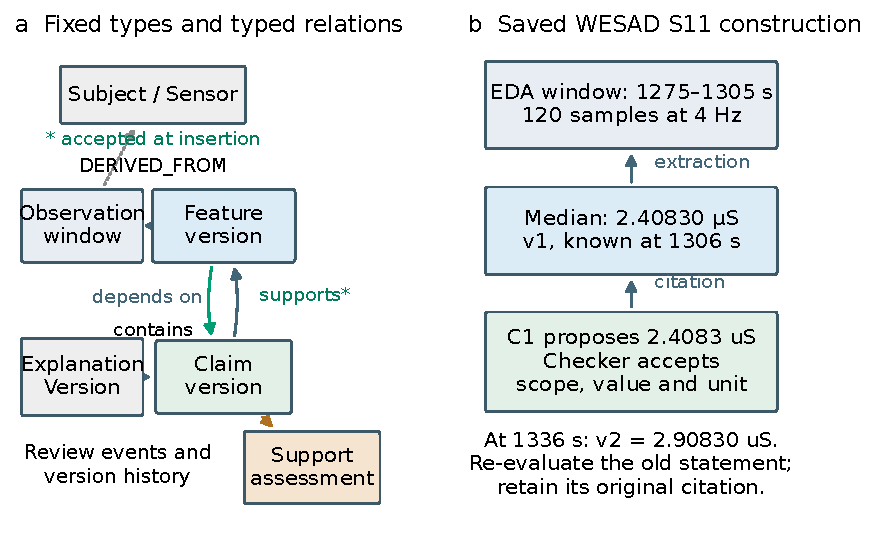
\includegraphics[width=\textwidth]{semantic_analysis_v1/ontology_construction.pdf}
\caption{Fixed vocabulary and an actual instance. Blue denotes deterministic
recording and feature construction, green a checked model proposition, grey
identity or display administration, and amber assessment or version effects.
The concrete path comes from the exported WESAD S11 correction scope.
Its source hash, sample indices and full IDs accompany the figure.
Arrows preserve stored direction. The schema shown is a readable subset of
the complete construction table.}
\label{fig:ontology}
\end{figure}

% start input ./generated/semantic/worked_example.tex
In the saved WESAD S11 episode (Figure~\ref{fig:ontology}), the electrodermal activity (EDA) window at 1275--1305 s produces a median of 2.408303 $\mu$S. The model proposes 2.408303 $\mu$S and cites that feature. The claim passes the bounded checks. Insertion records its \texttt{DEPENDS\_ON} citation and reverse \texttt{SUPPORTS} edge. A later feature version changes the median to 2.908303 $\mu$S, while the observation hash and original claim citation remain unchanged. Re-evaluation changes the claim's current support without rewriting its history.
 % end input ./generated/semantic/worked_example.tex

\subsection{Edges as Explicit Semantic Commitments}

An edge's type determines what it asserts. A citation names evidence offered as support. A parent link declares a prerequisite. An extraction edge records how
a feature was produced. Membership and co-occurrence imply neither support nor
a prerequisite. In particular, an LLM-proposed \texttt{DEPENDS\_ON} edge does not
prove that its target is necessary. \texttt{SUPPORTS} records acceptance when a
claim was inserted, not validity at every later time. \texttt{CONTRADICTS}
records an adverse assessment triggered by a revision, whose knowledge time is
stored in the associated assessment. Exports retain these origins and distinguish
proposed, accepted and displayed links.

\subsection{The Query-Specific Semantic Core}

To interpret and revise an answer, a reviewer needs its claims and the inputs
they cite. We select this semantic core by a fixed projection:
\begin{equation}
 K_{q,t}=\pi_{q,\Omega}(G_t),\qquad
 V(K_{q,t})=C_{q,t}^{*}\cup F_{q,t},\quad
 E(K_{q,t})=D_{q,t}\cup P_{q,t}.
\label{eq:core}
\end{equation}
$C_{q,t}^{*}$ contains the latest displayed answer's claims and their declared
claim ancestors. $F_{q,t}$ contains the visible feature propositions they cite,
including explicit availability watches. $D_{q,t}$ retains the corresponding
stored dependency edges. When a cited feature has a newer visible version,
$P_{q,t}$ records a labelled path from the original citation through the version
chain. Each such path keeps the citation and supersession witness IDs.
It is never drawn as a directly stored Neo4j relationship.

Linked metadata retains subject and sensor identities, explanation containers,
assessments and old versions. It also retains feature-to-observation provenance,
which can be expanded in the drawing. A claim's asserted fields determine its scope, not the wrapper's query interval. Full IDs,
raw sentences, original versions and assessment times remain recoverable.
The core preserves the answer's explicit commitments through this selection rule.

We analyze three distinct representations. The complete graph contains all stored
objects. The active projection at $t$ contains the latest evidence and current
display members across queries, with their observation provenance.
The core $K_{q,t}$ answers focused questions. Which window supports
a value, and which operands support a comparison? Which version was known,
what changed after correction, and does another witness still support the claim?
We evaluate these competency questions against immutable input logs or exact
program specifications, independently of database support flags.

% start input ./sections/review_view.tex
\subsection{Producing the Human-Review Network View}
\label{sec:reviewview}

The review view helps a reader trace a selected answer or claim back to its
evidence. It expands the semantic core with original cited versions, required
observation provenance and visible successor versions. Citations stay attached
to their original inputs. For a stored-node budget $B$ and selected recorded
times $T$, the transformation is
\begin{equation}
 H_{q,t}=\operatorname{View}_B(G_t,q),\quad
 p=\operatorname{Layout}\!\left(\bigcup_{u\in T}H_{q,u};m\right),\quad
 I_{q,t}=\operatorname{Render}(H_{q,t},p).
\label{eq:reviewview}
\end{equation}
$H$ is the bounded review expansion of $K$. The layout $p$ stores node coordinates
and routed edges, and rendering produces the drawing $I$.
Mode $m$ selects deterministic Graphviz \texttt{dot} for structured views or
seeded spring positioning for the classic network. Spring positioning uses an
undirected simple projection only to place nodes. Analysis and arrows retain
the typed directed graph. Routing and collision separation change presentation,
not support. Time comparisons reuse the layout of the union of their nodes.
Records not yet ingested remain absent from the earlier drawing. Coordinates
and distances do not measure semantic similarity or neural state.

The implementation selects a database scope, answer, focus and knowledge time,
then follows the declared inputs. It expands observation provenance on request.
Ingestion and assessment times determine visibility, while event intervals
describe when the measurements or assertions apply.
Original \texttt{DEPENDS\_ON} edges remain intact. A separate derived path records
how a citation resolves to a newer version, preserving the citation and the
supersession edges traversed in reverse. Availability, assessed support and
display membership remain separate. Among \SemAssessmentTies{} assessment groups
sharing a record and time, \SemAssessmentConflicts{} have conflicting states.
All outcomes and trigger IDs remain visible as ambiguous. Display membership
follows the saved explanation version. Neither flags nor drawings determine
the evaluator's reference truth.

The node budget favors complete sets of alternative witnesses when they fit.
Omitted records or incomplete witness groups produce a \emph{partial view}
warning and an expansion control. The view does not imply that omitted context
is irrelevant. Subject and sensor hubs, display containers, assessments and
reverse \texttt{SUPPORTS} edges remain in details. Structured views group feature
rows in labelled AND enclosures. Each row maps to a stored ID, and each dashed
bundle lists the original dependency edges it summarizes. These are drawing
constructs. All inputs within a witness are required, while different witnesses
are alternatives.

Green, blue and grey fills identify claims, features and observations.
Outlines and words identify revisions, support and withdrawal. Every arrow is
labelled with its stored direction or identified as a grouped edge.
Figures~\ref{fig:instances} and~\ref{fig:topology} share their typed JSON views,
ID maps and Graphviz renderer with the Streamlit dashboard.
Its optional \emph{Classic network} mode draws the same typed objects as individual
ellipses in Figure~\ref{fig:classic}. Selectboxes choose case, time, focus, witness
route and node or edge. Details show full sentences, exact values and units,
intervals, versions, source IDs and assessment provenance. Highlighting affects
appearance only. Expansion reveals omitted provenance, and review actions append
events in an isolated workspace. The interface makes external commitments
inspectable. It does not establish a human-performance benefit or reveal neural
reasoning.
 % end input ./sections/review_view.tex
  % end input ./sections/method.tex
 % start input ./sections/theory.tex
\section{Support, Locality and Transitive Exposure}
\label{sec:theory}

\subsection{Support Through Admissible Witnesses}

A claim remains supported if at least one valid route still justifies it.
For a proposition $c$, let $\mathcal W(c)$ be a finite family of admissible
witnesses. Each witness $W$ groups evidence or prerequisite propositions that
are jointly required. Different witnesses provide alternative routes:
\begin{equation}
 \operatorname{Supported}(c,t;q)=
 \bigvee_{W\in\mathcal W(c)}
 \left[\psi_c(W,t;q)\land
       \bigwedge_{u\in W}\operatorname{Valid}(u,t;q)\right].
\label{eq:support}
\end{equation}
A witness succeeds only when both checks pass.
$\operatorname{Valid}$ requires observable availability and admissible temporal
and subject scope. A prerequisite claim must itself be supported.
The predicate $\psi_c$ checks the asserted interval, selected logical versions,
quantity, normalized unit and numerical operation. Numerical agreement uses the
frozen tolerance $|v-\widehat v|\leq\max(10^{-6},0.01|\widehat v|)$.
A correction can make $\psi_c$ false while the source remains available. Historical and current assertions are different propositions. The extension's specified inequalities use exact floating-point comparisons.

The original model supports local AND/OR composition and a two-operand
difference. A generated numerical claim requires all its declared parents and
an admissible direct numerical witness. Comparisons cite both operands.
The extension represents alternatives as explicit lists of jointly required
inputs, connected through an acyclic positive claim graph. It does not support
unrestricted Boolean formulas. Each record's semantic-program metadata stores
the witness groups. Source IDs store their union for traversal, so edges alone
do not recover the AND/OR structure. To claim that evidence is missing, the
system needs a bounded set of possible producers and explicit availability
watches. Absence from an open graph is insufficient.

As in provenance and truth maintenance~\cite{green2007,doyle1979}, losing one
route need not remove support if another admissible witness survives.
Our alternatives use disjoint recording windows rather than renamed copies of
one measurement. These distinct sources need not be statistically independent.

\subsection{Locality of a Revision}

Reachable claims need checking, but need not change.
Let $U_\delta$ contain revised input identities, all earlier versions that can
still be cited, and any changed availability subscriptions. Dependency edges
point from a dependent to its input. Following them in reverse gives
\begin{equation}
 R_\delta=U_\delta\cup\operatorname{RevReach}(U_\delta),\qquad
 B_\delta=\{c:S_{t^-}(c)\ne S_{t^+}(c)\},
 \label{eq:locality}
\end{equation}
Here $S_t(c)$ abbreviates Equation~\ref{eq:support}.
$R_\delta$ contains changed inputs and reachable dependents for re-evaluation.
$B_\delta$ contains only claims whose support actually changes.

\begin{proposition}[Conditional locality]
For a finite acyclic dependency model, $B_\delta\subseteq R_\delta$ when every
mutable input to each support predicate is explicitly represented and only
$U_\delta$ changes between the two snapshots.
\end{proposition}
\noindent\emph{Proof sketch.}
Order nodes from inputs to dependents. A node outside $R_\delta$ has no changed
input or prerequisite in $R_\delta$, since either would make it reverse reachable.
Its scope, numerical operands and availability are unchanged. Induction in this
acyclic order gives unchanged prerequisite support and predicate values, hence
unchanged support. Including earlier versions covers citations to $v_1$ after
$v_2$ or $v_3$ arrives. Explicit availability records cover arrivals that falsify
an absence statement.\hfill$\square$

Unrecorded clock expiry, newly discovered witnesses without subscriptions, or
external predicate changes can violate locality. Our fixed-target queries and
controlled witness sets represent changes through version or availability events.
Benign updates and surviving alternatives show why the actual change set can be
strictly smaller than the candidate set, $B_\delta\subset R_\delta$.

Indexed adjacency traversal costs $O(|V_{R_\delta}|+|E_{R_\delta}|)$.
Current-version lookups, witness evaluation, snapshots, serialization, database
round trips and writes add to this cost. The original runtime repeatedly builds
version maps. Structural replay evaluates the whole small program before writing
scheduled updates. Neo4j variable-length queries may enumerate paths, whereas
SQLite uses a recursive SQL query with duplicate elimination. The abstract traversal
bound therefore gives neither implementation a linear-time guarantee.

\subsection{When Direct Maintenance Suffices}

Direct maintenance can miss changes to unscheduled claims.
Let $A_\delta$ be the independently determined set of prior admitted claims
requiring a state change, and $D_\delta$ the claims actually scheduled by direct-only
maintenance. For $|A_\delta|>0$, the fraction outside that schedule is
\begin{equation}
 \xi_\delta=\frac{|A_\delta\setminus D_\delta|}{|A_\delta|}.
 \label{eq:exposure}
\end{equation}
We report NA when $A_\delta$ is empty. The primary measure concerns withdrawal
of initially grounded claims. Restoration is recorded separately as a support
transition. The event-log/task oracle determines $A_\delta$ independently of
acceptance flags and graph paths.

\begin{proposition}[Direct/full equivalence and misses]
Assume initially correct states, complete re-evaluation of $D_\delta$, dependency
semantics consistent with the oracle, and no unrelated refresh or other mechanism
that revisits excluded claims. Before fresh generation, direct maintenance misses
the fraction $\xi_\delta$ of required changes. A sufficient condition for direct
and full maintenance to agree is that every changed support predicate is directly
scheduled. In particular, this holds when each changed input affecting an answer
has a direct dependency edge to every affected claim and all other predicates
remain unchanged.
\end{proposition}
\noindent\emph{Proof sketch.}
Complete direct re-evaluation changes every required member of $D_\delta$.
The no-refresh assumption leaves excluded members in their initial state.
The missed set is therefore exactly $A_\delta\setminus D_\delta$.
If all changed predicates are scheduled, both algorithms evaluate the same
predicates from the same snapshot. All remaining predicates retain equal
states.\hfill$\square$

Consider $c_1=$ ``test 1 holds'' and $c_2=$ ``tests 1 and 2 hold'', where $c_2$
requires $c_1$ and test 2. Correcting test 1 to false requires both claims to
change. A direct scheduler reaches only $c_1$, so $\xi_\delta=1/2$.
If $c_2$ also cites test 1 directly, the scheduler reaches it and exposure is zero.
If another independent route suffices for the answer, losing the first route
need not change the answer at all. Path length alone therefore predicts neither
a missed update nor a withdrawal. The waveform exports and controlled structural
experiment test these different cases.
 % end input ./sections/theory.tex
 % start input ./sections/design.tex
\section{Evaluation Design}
\label{sec:design}

\subsection{Preserved Three-Source Study}

The unchanged \texttt{minimum\_v1} study uses synthetic physiological-style
waveforms, WESAD laboratory recordings~\cite{schmidt2018,wesad}, and PPG-DaLiA
daily-activity recordings~\cite{reiss2019,ppgdalia}. Each source contributes ten
held-out subjects with two episodes each. The real-source splits use PCG64 seed
20260928 and five separate development subjects. Generation and checking exclude physiological and activity labels.
Outcomes concern recorded features.

Each episode has a 30-second target interval and a preceding 120-second
comparison interval. Four replay variants introduce clean or benign updates,
channel faults, delays and numerical corrections. Three knowledge checkpoints
occur at target end plus 1, 31 and 91 seconds. Four question families require
the target EDA median plus its preceding-window difference, EDA missing fraction
or acceleration variability. Requirements are fixed independently of answers.
Five methods produce 3,600 initial cases. B0 displays unchecked proposals.
B1 performs direct maintenance over indexed records, and B2 does so in Neo4j.
M1 uses Neo4j with transitive maintenance. B3 implements the same transitive
support rules in indexed SQLite with recursive common table expressions.
All checked methods use the same fresh-answer checks and at most one repair.

The original study uses pinned Qwen3-8B BF16~\cite{qwen3}, a three-claim contract and
1,536 output tokens. Both studies use the existing RTX 5090 and vLLM structured
decoding~\cite{vllm}, with model parameters and forward tensors verified on CUDA.
Database operations and statistics run on the host CPU. Neo4j Community 5.26
and indexed SQLite retain their adapters. The three original B0 transport
failures remain empty outputs.

\subsection{Independent Semantic Evaluation}

The \texttt{semantic\_analysis\_v1} oracle determines values and supporting
witnesses from immutable events and task specifications. It uses neither support
flags nor a neural verifier. Canonical proposition identity includes dataset,
subject, session, asserted interval, quantity, operation, normalized value and
unit, temporal mode and logical version. A correctly labelled background fact
can be grounded without answering the target question. Wrong numbers, subjects
and target attributions still fail. Citation and witness fidelity are separate from directly checkable truth.

Precision asks how much emitted content is grounded. Recall asks how many
answerable requirements it covers. For emitted checkable propositions $C(q,t)$
and answerable required propositions $R(q,t)$, we report
\begin{equation}
\begin{aligned}
 P_{\rm grounded}&=\frac{\sum_{c\in C}\mathbf 1[\text{source-grounded }c]}{|C|},\\
 R_{\rm required}&=\frac{|\{r\in R:\text{matched by a grounded }c\}|}{|R|}.
\end{aligned}
 \label{eq:semanticmetrics}
\end{equation}
Each requirement is counted once, so repeated paraphrases cannot increase recall.
The optional harmonic summary $S=2P_{\rm grounded}R_{\rm required}/
(P_{\rm grounded}+R_{\rm required})$ combines grounding and task completeness.
It is not conventional set F1 because their universes differ. For an answerable
question, empty output has precision NA and zero recall and summary score.
Fully unanswerable questions have recall and summary NA, with absence statements
checked separately. Partially answerable questions contribute their answerable facts.

We separately score raw and final proposals, accepted claims and displays.
A limited prose audit retains raw text, literal discrepancies and interpretation terms. Structured scores do not certify unrestricted language.
To assess temporal integrity, we score the same prior answer before arrival,
after arrival and after maintenance. These discrete checkpoints do not establish
a recovery curve. Withdrawing content and producing an adequate replacement
remain separate outcomes.

\subsection{Controlled Structural Extension}

Before new outputs are observed, \texttt{structure\_study\_v1} selects the first
five naturally sorted held-out subjects per source and both episodes.
These 30 episodes reuse participants rather than forming a new independent cohort.
Four intended evidence-to-answer depths (1--4) and two support regimes yield
240 cases. Each route compares EDA median, EDA interquartile range (IQR),
acceleration standard deviation (SD) and EDA missing fraction with explicit bounds.
The clean episode fixes these bounds so each route initially passes all four tests.
The answer states whether at least one eligible window passes all tests.
An alternative route uses the disjoint preceding window, which provides a distinct
observation witness for that existential statement. The task makes no physiological
diagnosis.

The depths group the same tests as direct inputs,
a complete route followed by an answer, a two-test prefix followed by a route and
answer, or a first test followed by that prefix, route and answer.
Exact compiled fixtures instantiate these programs. Separately, the model proposes
up to 16 claims and explicit witness lists, with 4,096 output tokens and at most
one repair. The compiler never fills in missing model links. We retain requested
and realized depth, omitted roots and incomplete alternative-witness families.
Two development pilots precede the core freeze. The second uses a generic grouping
example to clarify readable sentences and reuse of emitted parent IDs.
Neither pilot inserts required links. Both use development episodes, and their
40 calls are separate from the core budget.

Each method replays the same admitted candidate without generation after
correction. B0 here disables maintenance on that content.
Four independent update conditions make the first test false in every route,
remove only the primary route, make a benign numerical change, or revise an
unused cardiac feature. Neo4j and relational methods receive identical candidates,
events and predicates. An independent truth-table evaluator enumerates the bounded
Boolean assignments to test witness entailment and equivalence, allowing different
valid derivations. A separate event-log evaluator determines required changes.

\subsection{Graph Measurement and Uncertainty}

Read-only Neo4j exports preserve nodes, relations, assessment times, Cypher and
element IDs. Counts match the original ledger and sampled stored paths.
Separate measurements of the full graph, active graph and query core cover type mixing, degree, depth, direct citations, witness counts, reachability
and actual changes. Dependency degree excludes SUPPORTS and provenance mirrors.
Meaningful zero categories remain, and we impose no power-law or embedding
interpretation.

We first aggregate snapshots and variants within episodes, then episodes within
subjects. Pointwise 95\% intervals use 2,000 subject-cluster bootstrap resamples
with seed 20260929. Historical versions and replay copies never count as
independent participants. Detailed distributions and operational logs remain
repository data. This paper retains the definitions and primary denominators
needed to interpret the results.
 % end input ./sections/design.tex
 % start input ./sections/results.tex
\section{Results}
\label{sec:results}

\subsection{Storage Structure and Semantic Structure Differ}

The export covers \SemExportScopes{} retained Neo4j scopes. Counts match the
original ledger, and \SemVerifiedPaths{} representative stored paths are verified.
M1 stores \SemStorageNodes{} nodes and \SemStorageEdges{} relations across its
replay scopes. These totals measure storage, not independent observations.
Membership and extraction rules create many of the edges. Neither these edges
nor the reverse links added when claims are accepted imply deeper reasoning.

Across sources, the query core averages \SemCoreSizeMin--\SemCoreSizeMax{} nodes,
or \SemCoreRatioMin--\SemCoreRatioMax\% of visible storage. It is smaller because
it selects answer propositions and their declared inputs. The active graph also
contains other visible evidence. Linked metadata preserves the observation
witnesses. Full storage counts include historical versions, whereas core sizes
count visible propositions for each query. Aggregating within subjects prevents
replay copies from being treated as independent samples.

\begin{figure}[p]
\centering
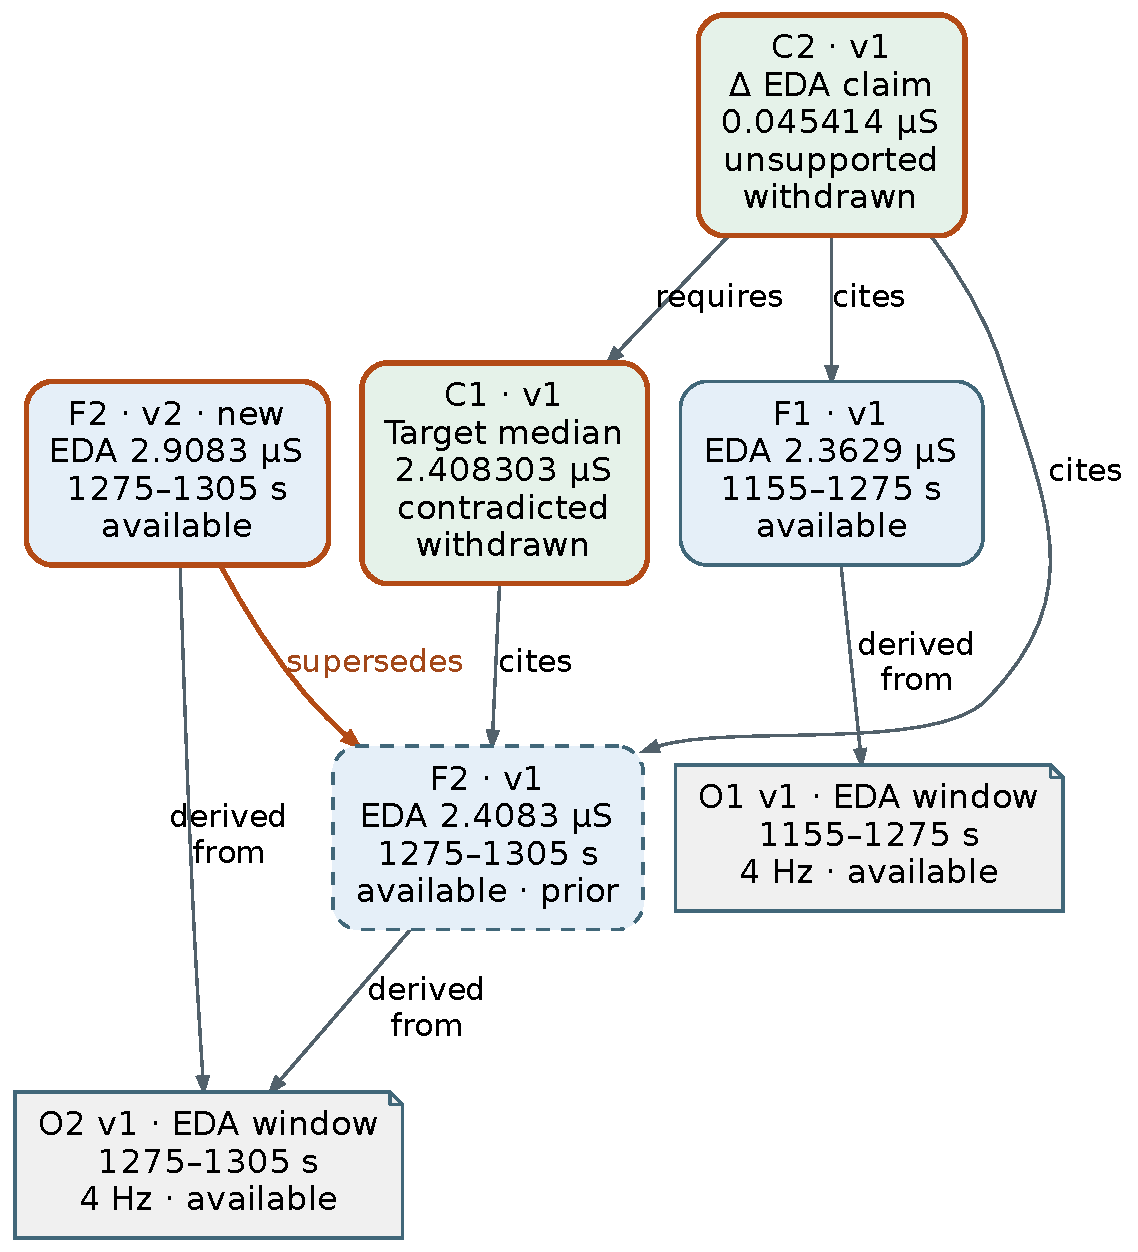
\includegraphics[width=\textwidth]{semantic_analysis_v1/real_revision_network.pdf}
\caption{Review network from actual Neo4j records for WESAD S11, episode 0,
at knowledge time \ViewRealAfter{} s. The unchanged median-size rule selects this
case among \ViewRealEligible{} eligible correction cores. Green nodes are claims,
blue nodes are features, and folded corners mark observations. \emph{Cites/requires}
mean \texttt{DEPENDS\_ON}, \emph{derived from} means \texttt{DERIVED\_FROM}, and
\emph{supersedes} points from new to old. The injected correction adds F2 v2.
C1/C2 retain their original v1 citations and are withdrawn. Availability remains
distinct from current support. C2 cites both operands directly, so direct checking
suffices. Identity hubs, admission mirrors and assessment/display containers are
hidden but inspectable in details. Labels round values, while metadata preserves
full precision.}
\label{fig:instances}
\end{figure}

\begin{figure}[p]
\centering
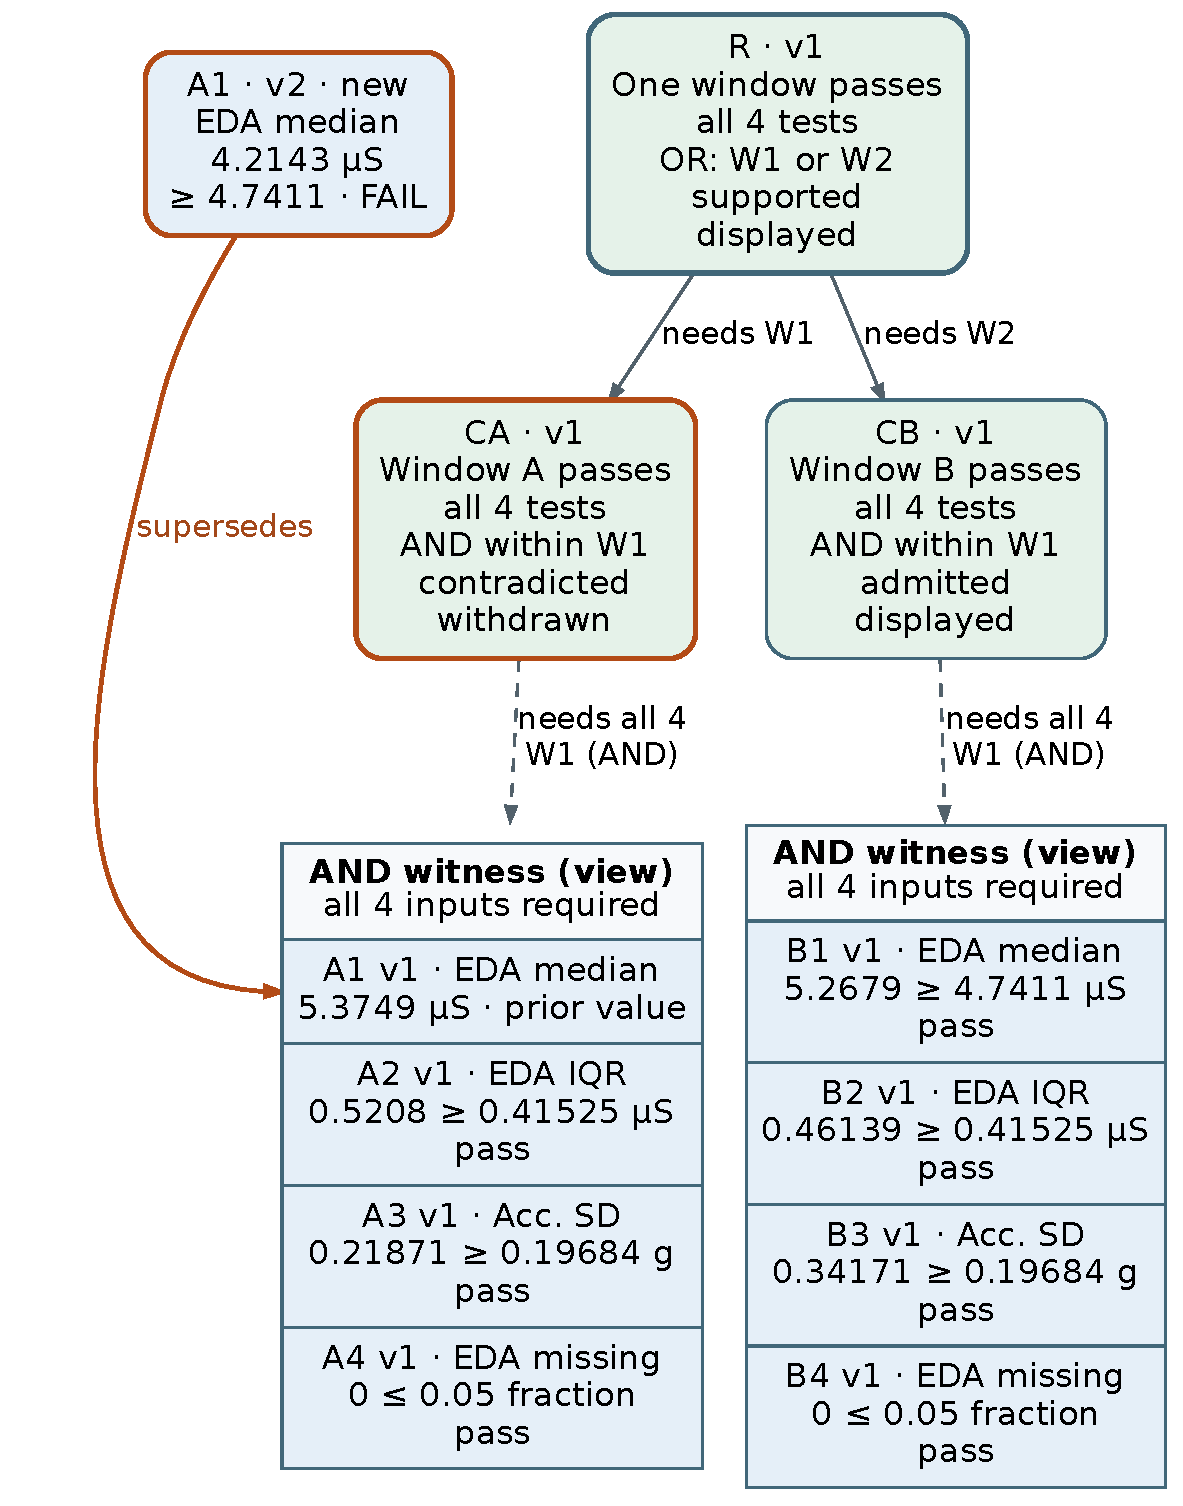
\includegraphics[width=\textwidth]{semantic_analysis_v1/structural_witness_network.pdf}
\caption{Generated program from Neo4j for PPG-DaLiA S1 episode 0
at knowledge time \ViewStructAfter{} s. Requested and realized depth are both
\ViewStructDepth{}. The smallest complete graph among
\ViewStructEligible{} eligible programs is selected, with ties broken by ID. Windows A/B span
\ViewRouteAInterval/\ViewRouteBInterval{} s. Correcting A1 invalidates CA, but
CB still supports R. Alternative routes W1/W2 each require all four inputs.
Blue rows are stored features. Dashed bundles summarize four \texttt{DEPENDS\_ON}
edges. AND enclosures are drawing constructs with exported row/edge mappings.
Solid \emph{needs} arrows are stored parent dependencies. Observation provenance
expands on request. Administrative details remain inspectable.}
\label{fig:topology}
\end{figure}

% Keep the interpretation together after the two network pages.
\clearpage
Only \SemParentClaims{} of \SemDisplayedClaims{} displayed M1 claims declare a
parent, leaving \SemParentlessPercent\% parentless. Claim-parent depth never
exceeds one. Even a parent edge need not create transitive exposure.
In Figure~\ref{fig:instances}, the comparison also cites the corrected feature
directly. Of \SemRevisionBatches{} revision batches, \SemEligibleBatches{} require
a withdrawal and \SemNonzeroExposure{} have nonzero exposure. The locality audit
finds \SemLocalityViolations{} violations. These dependencies explain why
direct and full maintenance agree. The equivalence does not arise from missing
stored paths or a particular database engine.

% start input ./sections/classic_case.tex
\paragraph{A worked ontology instance.}
Figure~\ref{fig:classic} shows how the ontology in
Equations~\ref{eq:ontology}--\ref{eq:construction} represents the admitted
PPG-DaLiA program. A1 is a particular \texttt{FeatureVersion} instance, not the
feature class itself. The drawing shows \ClassicNodes{} records and
\ClassicEdges{} stored relations from a scope of \ClassicScopeNodes{} objects
and \ClassicScopeEdges{} relations. Its \ClassicCore{} starred records form the
current core in Equation~\ref{eq:core}. CA remains a declared ancestor of R,
although CA has been withdrawn from the displayed answer. Old A1 and the two
EDA windows provide review context. Motion-window provenance can be expanded.

Each route requires four tests, and either route can support the answer.
For this program, Equation~\ref{eq:support} becomes
% start input ./generated/classic_network/witness_expression.tex
\[
\begin{aligned}
S(C_{A},t)&=b_{A1}(t)\land b_{A2}(t)\land b_{A3}(t)\land b_{A4}(t)\\S(C_{B},t)&=b_{B1}(t)\land b_{B2}(t)\land b_{B3}(t)\land b_{B4}(t)\\S(R,t)&=S(C_{A},t)\lor S(C_{B},t)
\end{aligned}
\]
 % end input ./generated/classic_network/witness_expression.tex
 Each $b_{ri}$ checks the latest visible feature for PPG-DaLiA S1, session 1,
with the specified A/B interval, quantity and unit and an available non-null value.
It then applies the exact $\geq$ threshold for median, IQR and acceleration SD,
or $\leq$ for missing fraction (Figure~\ref{fig:topology}). A1 changes from
\ClassicOldValue{} $\mu$S, above \ClassicThreshold{} $\mu$S, to
\ClassicNewValue{} $\mu$S, below it. The measurement remains available, but
$b_{A1}$ becomes false. The witness lists therefore give
$(S(C_A),S(C_B),S(R)): (1,1,1)\to(0,1,1)$.

The theorem's dependency projection contains \ClassicDependencyNodes{} nodes
and \ClassicDependencyEdges{} edges. Reachability excludes provenance, membership
and support mirrors. Equation~\ref{eq:locality} gives
$U_\delta=\{\mathrm{A1}_{v1},\mathrm{A1}_{v2}\}$ and
$R_\delta=U_\delta\cup\{C_A,R\}$, but $B_\delta=\{C_A\}$.
These full computed sets are all visible here. The independent event/task oracle
and recorded B2 schedule separately give $A_\delta=D_\delta=\{C_A\}$.
Exposure in Equation~\ref{eq:exposure} is $0/1=0$.
Two dependent claims need re-evaluation, yet only CA changes support because
another witness preserves the root. Direct and full maintenance agree.

\begin{figure}[p]
\centering
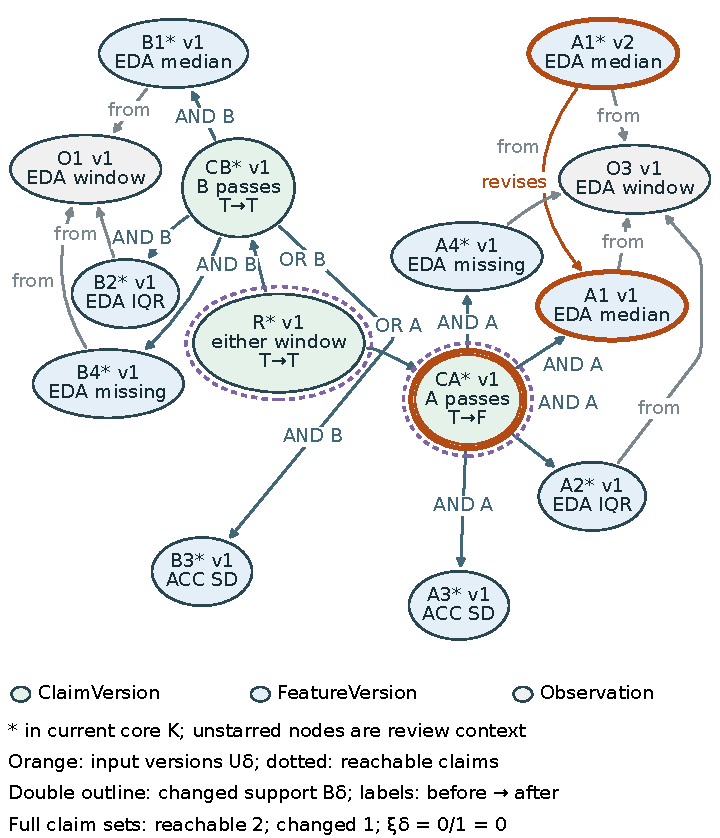
\includegraphics[width=\textwidth]{semantic_analysis_v1/ontology_instance_network.pdf}
\caption{Classic ontology-instance view of the admitted program
\texttt{ppg\_dalia-S1-e0-d2-alternative}, PPG-DaLiA S1 episode 0.
The primary route is corrected at \ClassicArrival{} s. The view compares
\ClassicAfter{} s with \ClassicBefore{} s. All \ClassicNodes{} ellipses are
stored records. AND A/B identify the four jointly required inputs of CA/CB.
OR A/B identify R's alternative parent witnesses. Both mean \texttt{DEPENDS\_ON}.
\emph{From} means \texttt{DERIVED\_FROM}, and \emph{revises} means new-to-old
\texttt{SUPERSEDES}. Original citations remain intact. Motion windows,
administrative relations, feature dependency duplicates and \texttt{SUPPORTS}
mirrors are hidden. Fill identifies ontology class. Outlines and stars show
computed revision sets and core membership. Visual annotations add no database
nodes or dependencies.}
\label{fig:classic}
\end{figure}
 % end input ./sections/classic_case.tex

\subsection{Grounded Content and Useful Coverage}

\begin{table}[!htbp]
\caption{Independent semantic scores in percent (subject means and 95\% intervals).
Each row contains 240 answer instances from 20 episodes. Matched counts unique
requirements within each answer. Denominators count answerable requirements.
Empty displays have zero recall on answerable questions and undefined precision.
The original strict-contract interpretation is preserved separately from these scores.}
\label{tab:fidelity}
\centering\scriptsize\setlength{\tabcolsep}{3pt}
% start input ./generated/semantic/fidelity_table.tex
\begin{tabular}{llrrrr}
\toprule
Source & State & $P$ [95\% CI] & $R$ [95\% CI] & Matched & Empty \\
\midrule
Synthetic & B0 display & 87.8 [84.5, 90.5] & 95.5 [90.0, 99.5] & 402/420 & 1 \\
Synthetic & M1 raw & 87.3 [83.4, 90.4] & 95.0 [88.5, 100.0] & 400/420 & 0 \\
Synthetic & M1 display & 100.0 [100.0, 100.0] & 78.2 [66.2, 90.0] & 333/420 & 20 \\
WESAD & B0 display & 83.6 [77.2, 89.4] & 86.5 [77.8, 95.0] & 366/420 & 1 \\
WESAD & M1 raw & 83.4 [77.1, 89.2] & 87.0 [78.2, 95.5] & 368/420 & 0 \\
WESAD & M1 display & 100.0 [100.0, 100.0] & 75.8 [64.0, 87.5] & 323/420 & 20 \\
PPG-DaLiA & B0 display & 84.5 [78.7, 89.6] & 87.8 [79.2, 94.8] & 371/420 & 1 \\
PPG-DaLiA & M1 raw & 84.7 [79.2, 89.6] & 88.8 [80.7, 95.5] & 375/420 & 0 \\
PPG-DaLiA & M1 display & 100.0 [100.0, 100.0] & 75.5 [65.0, 87.5] & 322/420 & 20 \\
\bottomrule
\end{tabular}
 % end input ./generated/semantic/fidelity_table.tex
\space% Preserve the former table-input boundary.
 \end{table}

\begin{figure}[!htbp]
\centering
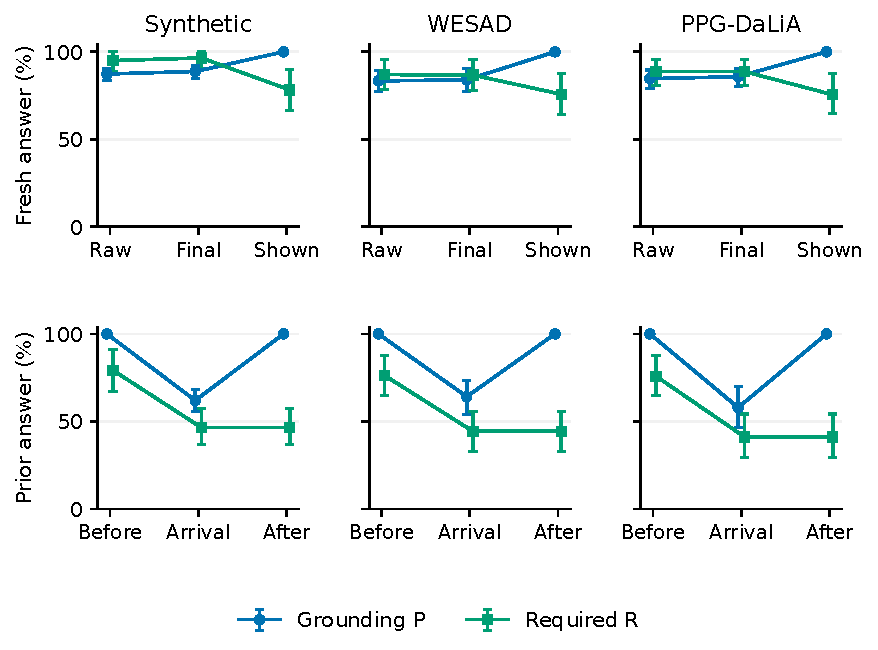
\includegraphics[width=\textwidth]{semantic_analysis_v1/semantic_fidelity.pdf}
\caption{Independent grounding precision and required recall for the same prior
M1 answers at three discrete checkpoints, with subject-cluster 95\% intervals.
Each source has 160 transitions from 20 episodes and ten subjects across the
four variants. No smooth recovery curve is inferred. Emitted-claim and required-fact
denominators appear in the text. Fresh-answer scores remain in
Table~\ref{tab:fidelity}.}
\label{fig:fidelity}
\end{figure}

% start input ./generated/semantic/temporal_denominators.tex
Emitted-claim counts before arrival, after arrival and after maintenance are Synthetic 211/211/138, WESAD 281/281/207, and PPG-DaLiA 271/271/191. Each source has 260/290/290 answerable required facts at these checkpoints. Precision excludes empty outputs, whereas recall includes their zero coverage. These pooled counts describe the sample. Reported percentages average episodes within subjects.
 % end input ./generated/semantic/temporal_denominators.tex

Checking produces fully grounded displays under the bounded numerical protocol,
but it also removes useful information.

Raw M1 required recall is
\SemSyntheticRawR\%, \SemWesadRawR\% and \SemPpgRawR\% for synthetic, WESAD and
PPG-DaLiA respectively. Displayed recall falls to \SemSyntheticDisplayR\%,
\SemWesadDisplayR\% and \SemPpgDisplayR\% (Table~\ref{tab:fidelity}).
Thus the precision gain partly comes from rejecting correct, useful propositions.
Figure~\ref{fig:fidelity} follows the same prior answers.
Withdrawing stale assertions restores grounding among retained claims, but
required facts can remain unanswered.

Of \SemContractInvalid{} B0 claims rejected by the frozen contract,
\SemInvalidGrounded{} are grounded under the new proposition protocol.
This includes \SemBackground{} correctly time-labelled background observations.
Other disagreements arise when dependency or citation restrictions reject
correct numerical content. No claim that passed the old contract becomes
numerically ungrounded under the new scoring. A wrong target attribution still
fails because matching uses the asserted interval and independently resolved version.

Queries about source windows and known versions agree with the independent log
oracle on all \SemCompetencyWitnesses{} feature witnesses. Queries about comparison
operands agree on \SemCompetencyComparisons{} eligible displayed comparisons.
These checks recover admissible witnesses without requiring a unique gold
reasoning graph. The separate prose audit and
original auxiliary-verifier disagreements remain available. The bounded scores
do not certify unrestricted interpretation.

\subsection{Structural Variation Tests the Maintenance Condition}

\begin{figure}[!htbp]
\centering
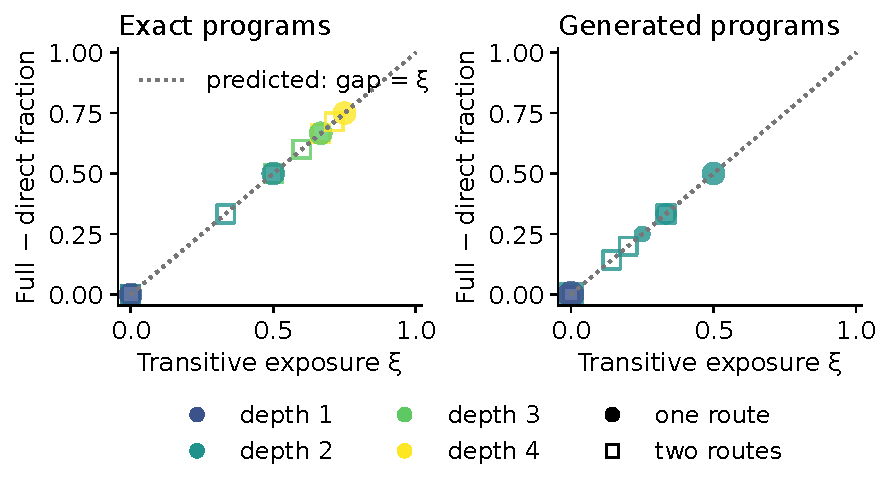
\includegraphics[width=\textwidth]{semantic_analysis_v1/structural_theory_test.pdf}
\caption{Population-level structural test. Full-minus-direct correction fraction
versus independently computed transitive exposure, separately for exact compiled
and admitted GPU-generated programs. Points aggregate equal exposure, support
regime and realized depth. Size reflects batch count, and the diagonal shows the
conditional prediction. These are primary-admission results. The text reports
the separate sensitivity analysis after normalization.}
\label{fig:structure}
\end{figure}

\begin{table}[!htbp]
\caption{Common-candidate structural replay. Counts aggregate four update conditions
per case, separately for exact and generated programs. A required change is
independently determined before scheduling. Correction intervals average episodes
within subjects identified separately for each dataset. B1 matches B2 and B3 matches M1 in every cell.
Missing generated roots are included in the depth/coverage analysis, not invented
as initially displayed claims.}
\label{tab:structural}
\centering\small\setlength{\tabcolsep}{4pt}
% start input ./generated/semantic/structural_table.tex
\begin{tabular}{llrrrr}
\toprule
Program & Method & Required & Missed & Collateral & Corrected \% [CI] \\
\midrule
Exact & B0 & 1260 & 1260 & 0 & 0.0 [0.0, 0.0] \\
Exact & B2 & 1260 & 720 & 0 & 42.9 [42.9, 42.9] \\
Exact & M1 & 1260 & 0 & 0 & 100.0 [100.0, 100.0] \\
Generated & B0 & 1210 & 1210 & 0 & 0.0 [0.0, 0.0] \\
Generated & B2 & 1210 & 183 & 0 & 84.9 [84.0, 85.7] \\
Generated & M1 & 1210 & 0 & 0 & 100.0 [100.0, 100.0] \\
\bottomrule
\end{tabular}
 % end input ./generated/semantic/structural_table.tex
\space% Preserve the former table-input boundary.
 \end{table}

The extension produces \SemCoreCases{} common candidates with \SemCoreCalls{}
GPU calls, including \SemCoreRepairs{} repairs, in \SemCoreMinutes{} minutes.
Its \SemReplayCells{} replays include exact and generated programs. Neo4j and the relational control agree in all \SemParityGroups{}
matched groups of program origin and update. Direct maintenance misses
\SemFixtureMissed{} of \SemFixtureRequired{} required changes in exact programs
and \SemGeneratedMissed{} of \SemGeneratedRequired{} in admitted generated programs.
Full maintenance misses none and withdraws no unaffected claims.
Predicted misses agree in all \SemPredictionAgreement{} of
\SemPredictionGroups{} eligible groups (Figure~\ref{fig:structure}).

Generated answers have depth one in \SemRootOne{} cases and depth two in
\SemRootTwo{} cases.
Another \SemMissingRoots{} cases have no admitted answer root. None reaches depth
three or four. The model usually proposes route claims followed by an answer.
Exact programs test deeper counterexamples, while generated programs test the
expressed dependencies. When the primary route is
lost, all \SemFixtureAlternative{} exact and \SemGeneratedAlternative{} generated
two-route answers with admitted roots remain supported. Single-route roots do not.
In Figure~\ref{fig:topology}, A1 changes from
\ViewRouteOld{} to \ViewRouteNew{} $\mu$S, below its \ViewRouteThreshold{} $\mu$S
threshold. CA is withdrawn, but CB and the answer remain displayed.
Direct and full maintenance agree for this update. Other tested conditions require updates to dependents excluded by direct scheduling.
Necessary dependencies and surviving alternatives determine the outcome, not path length. In \SemSameSize{} paired cases, programs with
the same evidence and baseline record count have different exposure.
Storage size alone therefore cannot explain maintenance behavior.

After the core run, we found an omission in the admission table. Primitive test
names were defined in the input but unavailable as claim proposition names.
This produced \SemUnknownPrimitive{} unknown-proposition rejection reasons.
A separate corrected replication maps those names to their supplied comparators
without changing candidates, witnesses or links. It admits \SemAliasRoots{} roots
and repeats \SemAliasCells{} CPU database replays. Direct maintenance misses
\SemAliasMissed{} of \SemAliasRequired{} required changes, while full maintenance
again misses none. The original scores remain frozen. Truth-table scoring independently distinguishes
initially true statements from sound, complete witness families. This admission
correction adds no model reasoning.

\subsection{Operational Cost and Adequate Replacement}

The original systems workload produces \SystemsAdequate{} adequate replacements
among \SystemsExplanations{} completed candidates. All omit the required preceding-window difference, so no successful
replacement time is observed. At the highest offered rate, both databases accumulate a backlog and
delay flags. The extension maintains a common answer without post-correction generation.
It establishes selective withdrawal and preservation, not an adequate replacement.
Replay timings include diagnostic traversal and whole-program evaluation.
They measure instrumented costs rather than production latency.
 % end input ./sections/results.tex
 % start input ./sections/discussion.tex
\section{Discussion and Conclusion}

The representation distinguishes a changed value, an invalid prerequisite and a
surviving witness. The ontology defines these commitments,
and the review view exposes their evidence and versions. Locality limits which
claims need re-evaluation. Transitive exposure identifies required changes that
direct scheduling excludes. The two measured regimes show why declared paths
and requested depth alone do not establish a maintenance advantage.

Withdrawing stale content can preserve grounding while leaving required facts
unanswered. A strict contract can also reject correct background information.
Independent proposition and witness scores distinguish these outcomes.
Admission normalization changes which supplied definitions the checker recognizes
without changing model outputs or parent links.

The findings concern bounded propositions, fixed witness sets and acyclic
dependencies. Agreement with recordings does not establish physiological truth.
Natural faults, clock expiry, open-ended evidence discovery and unrestricted
prose need further study. Generalization is limited by ten held-out subjects per
source, five reused in the extension, one generator and one seed. Disjoint windows
are not statistically independent. Neo4j and the relational control agree on
matched updates, without establishing a universal ranking of storage performance.
The dashboard supports event-driven inspection and isolated review actions.
Human decision accuracy, interaction latency and real-time benefit remain untested.
The original failure to produce adequate replacements limits recovery claims.

\paragraph{Artifacts.}
The repository preserves frozen studies, raw candidates, independent scores,
database exports, shared review views, vector figures, reproduction commands and
exhaustive logs. All essential definitions and sensitivity results appear here.
Provider recordings are not redistributed.

\paragraph{Use of generative AI.}
An AI coding assistant supported implementation, analysis and drafting.
Qwen3-8B generated candidates, and Qwen2.5-3B-Instruct supplied the auxiliary audit.
Human authors must review the evidence and interpretations before submission.
 % end input ./sections/discussion.tex
 \clearpage
\label{page:references}
\begin{thebibliography}{10}
\providecommand{\url}[1]{\texttt{#1}}
\providecommand{\urlprefix}{URL }
\providecommand{\doi}[1]{https://doi.org/#1}

\bibitem{doyle1979}
Doyle, J.: A truth maintenance system. Artificial Intelligence  \textbf{12}(3),
   231--272 (1979). \doi{10.1016/0004-3702(79)90008-0}

\bibitem{edge2025}
Edge, D., Trinh, H., Cheng, N., Bradley, J., Chao, A., Mody, A., Truitt, S.,
  Metropolitansky, D., Ness, R.O., Larson, J.: From local to global: A graph
  {RAG} approach to query-focused summarization (2025),
  \url{https://arxiv.org/abs/2404.16130v2}, version 2

\bibitem{green2007}
Green, T.J., Karvounarakis, G., Tannen, V.: Provenance semirings. In:
  Proceedings of ACM PODS. pp. 31--40 (2007). \doi{10.1145/1265530.1265535}

\bibitem{gupta1993}
Gupta, A., Mumick, I.S., Subrahmanian, V.S.: Maintaining views incrementally.
  In: Proceedings of ACM SIGMOD. pp. 157--166 (1993).
  \doi{10.1145/170035.170066}

\bibitem{qwen3}
{Qwen Team}: {Qwen3-8B} model card (2025),
  \url{https://huggingface.co/Qwen/Qwen3-8B}, revision
  b968826d9c46dd6066d109eabc6255188de91218

\bibitem{rasmussen2025}
Rasmussen, P., Paliychuk, P., Beauvais, T., Ryan, J., Chalef, D.: Zep: A
  temporal knowledge graph architecture for agent memory (2025),
  \url{https://arxiv.org/abs/2501.13956}

\bibitem{ppgdalia}
Reiss, A., Indlekofer, I., Schmidt, P.: {PPG-DaLiA}. UCI Machine Learning
  Repository (2019). \doi{10.24432/C53890}

\bibitem{reiss2019}
Reiss, A., Indlekofer, I., Schmidt, P., Van~Laerhoven, K.: Deep {PPG}:
  Large-scale heart rate estimation with convolutional neural networks. Sensors
   \textbf{19}(14), ~3079 (2019). \doi{10.3390/s19143079}

\bibitem{wesad}
Schmidt, P., Reiss, A.: {WESAD} (wearable stress and affect detection). UCI
  Machine Learning Repository (2018). \doi{10.24432/C57K5T}

\bibitem{schmidt2018}
Schmidt, P., Reiss, A., Duerichen, R., Marberger, C., Van~Laerhoven, K.:
  Introducing {WESAD}, a multimodal dataset for wearable stress and affect
  detection. In: Proceedings of the International Conference on Multimodal
  Interaction. pp. 400--408 (2018). \doi{10.1145/3242969.3242985}

\bibitem{turpin2023}
Turpin, M., Michael, J., Perez, E., Bowman, S.R.: Language models don't always
  say what they think: Unfaithful explanations in chain-of-thought prompting.
  In: Advances in Neural Information Processing Systems (2023),
  \url{https://arxiv.org/abs/2305.04388}

\bibitem{vllm}
{vLLM Contributors}: Structured outputs (2025),
  \url{https://docs.vllm.ai/en/v0.10.2/features/structured_outputs.html},
  version 0.10.2

\bibitem{prov2013}
{W3C PROV Working Group}: {PROV-DM}: The {PROV} data model. {W3C}
  recommendation, World Wide Web Consortium (April 2013),
  \url{https://www.w3.org/TR/prov-dm/}

\end{thebibliography}

\end{document}
